\section{Auswertung}


\subsection{Bestimmung der Kugeldichten}

In Tabelle \ref{tab:messwerte_kugel} sind die gemessenen Radien und Masses der Kugel 
einzusehen.

\begin{table}
\centering
\begin{tabular} {ccccccc}
	\toprule
  & \multicolumn{3}{c}{Radius in $\si{\meter}\cdot \num{e-3}$}  & \multicolumn{3}{c}{Masse in $\si{\kilogram}\cdot \num{e-3}$} \\
\midrule \\
Kugel 1 & $\num{7.565} $&  $\num{7.5625} $ & $\num{7.565} $  & $\num{4.45}$ & $\num{4.44} $ & $\num{4.44} $ \\
Kugel 2  & $\num{7.65} $&  $\num{7.65} $ & $\num{7.65} $ & $\num{4.6}$ & $\num{4.6} $ & $\num{4.61} $ \\
\bottomrule
\end{tabular}
\caption{Abmessung der Kugeln}
\label{tab:messwerte_kugel}
\end{table}

Der Mittelwert der Messreihen wird mittels

\begin{equation}
\label{eq:mittel}
\bar{x}=\frac{1}{n}\sum_{i=1}x_i
\end{equation}

berechnet. Dabei wird der zugehörige Fehler
durch 
\begin{equation}
\label{eq:stand_ab}
\bar{\sigma}_{\bar{x}}=\sqrt{\frac{1}{n(n-1)}\sum_{i=1}^{n}(x_i-\bar{x})^2}.
\end{equation}

bestimmt.

Für die Messungen aus \ref{tab:messwerte_kugel} ergeben sich 
folgende gemittelten Werte:

\begin{align}
\label{eq:abmessungen_kugel}
\begin{aligned}
\overline{m}_{1}&= \left(\num{0.0044}\pm\num{e-6}\right) \si{\kilogram} \\
\overline{m}_{2}&= \left(\num{0.0046}\pm\num{e-6}\right) \si{\kilogram} \\
\hfill \\
\overline{r}_{1}&= \left(\num{0.0076}\pm\num{e-7}\right) \si{\meter} \\
\overline{r}_{2}&= \left(\num{0.0077}\pm\num{0}\right) \si{\meter} \\
\end{aligned}
\end{align}

Mithilfe der gemittelten Werte und der Formel

\begin{equation*}
\rho=\frac{m}{V_{k}} \qquad \text{mit} \, V_{k}=\frac{4}{3}\pi r^3
\end{equation*}

können die Dichten der Kugeln bestimmt werden.
Es ergibt sich:

\begin{align*}
\rho_{1}&=\left(\num{2451.0}\pm\num{1.6}\right) \si{\kilogram\per\cubic\meter}\\
\rho_{2}&=\left(\num{2454.7}\pm\num{1.5}\right) \si{\kilogram\per\cubic\meter}
\end{align*}

\subsection{Bestimmung der Viskosität von Wasser bei Zimmertemperatur} \label{sec:visko}
Um die Viskosität zu bestimmen wird neben der Dichte von Wasser die Fallzeit von der kleinen Kugel benötigt.
Die gemessenen Werte sind in Tabelle \ref{tab:messwerte_fallzeit_kugel_klein} abgebildet. 
\begin{table}
\centering
\begin{tabular} {c}
	\toprule
  Fallzeit $t_1$ in $\si{\second}$ \\
  \midrule
  $\num{12.7}$ \\
  $\num{12.8}$ \\
  $\num{12.9}$ \\
  $\num{12.8}$ \\
  $\num{12.8}$ \\
  $\num{12.8}$ \\
  $\num{12.7}$ \\
  $\num{12.7}$ \\
  $\num{12.7}$ \\
  $\num{12.8}$ \\
\bottomrule
\end{tabular}
\caption{Fallzeiten der kleinen Kugel im Viskosimeter bei $\SI{20}{\degreeCelsius}$}
\end{table}

Gemittelt ergibt sich

\begin{equation}
\label{eq:gemittelte_fallzeit_klein}
\overline{t}_{1}=\left(\num{12.78}\pm\num{0.02}\right) \si{\second}.
\end{equation}
Mittels der Gleichung \eqref{eq: eta} ergibt sich als Viskosität
für Wasser bei $\SI{20}{\degreeCelsius}$:

\begin{equation}
\label{eq:viskosi_wasser}
\eta_{20}=\left(\num{0.0014}\pm\num{e-5}\right) \si{\pascal\second}
\end{equation}

Für die Dichte von Wasser bei $\SI{20}{\degreeCelsius}$ wurde als
Literaturwert $\rho_{20}=\SI{998.21}{\kilogram\per\cubic\meter}$ angenommen. %Wichtig: Literaturverweis angeben

\subsection{Bestimmungen der Apperaturkonstante für die große Kugel}
Um die Apperaturkonstante für die große Kugel zu bestimmen nutzt man die 
Gleichung \eqref{eq: eta}. Diese wird umgestellt zu 

\begin{equation*}
\Leftrightarrow \quad K_{g}=\frac{\eta}{\left(\rho_2-\rho_{20}\right)\overline{t}_2}
\end{equation*}

Hierbeisei $)\overline{t}_2$ die Fallzeit der zweiten Kugel im Viskosimeter.
Die aufgenommenen Messwerte sind in Tabelle \ref{tab:messwerte_fallzeit_kugel_gross} dargestellt.

\begin{table}
\centering
\begin{tabular} {c}
  \toprule
  Fallzeit $t_2$ in $\si{\second}$ \\
  \midrule
  $\num{97.3}$ \\
  $\num{97.6}$ \\
  $\num{97.4}$ \\
  $\num{97.8}$ \\
  $\num{97.2}$ \\
  $\num{97.3}$ \\
  $\num{97.2}$ \\
  $\num{97.3}$ \\
  $\num{97.6}$ \\
  $\num{97.7}$ \\
\bottomrule
\end{tabular}
\caption{Fallzeiten der großen Kugel im Viskosimeter bei $\SI{20}{\degreeCelsius}$}
\label{tab:messwerte_fallzeit_kugel_gross}
\end{table}

Als gemittelte Zeit ergibt sich:
\begin{equation}
\label{eq:gemittelte_fallzeit_gross}
\overline{t}_{2}=\left(\num{97.44}\pm\num{0.07}\right) \si{\second}.
\end{equation}

Mit dem Ergebnis aus \eqref{eq:viskosi_wasser} folgt für die 
Apperaturkonstante

\begin{equation}
\label{eq:app_konst_gross}
K_{g}=\left(\num{9.98}\pm\num{0.02}\right)\cdot{\num{e-9}} \si{\pascal\cubic\meter\per\kilogram}
\end{equation}

\subsection{Bestimmung der Viskosität in Abhängigkeit von der Temperatur}

Das prinzipielle Verfahren zu Berechnung der Viskosotät $\eta$ ist
das Selbe, wie im Unterkapitel \ref{sec:visko}.
Lediglich die Dichte von Wasser ist nicht mehr konstant.
Als Dichte des Wasser wurden folgende Dichten angenommen:  %Noch literatur ref

\begin{table}
\centering
\begin{tabular} {cc}
  \toprule
  Temperatur in $\si{\kelvin}$ & Dichte $\rho$ in $\si{\kilogram\per\cubic\meter}$ \\
  \midrule
  $\num{303.16}$ &$\num{995.65}$ \\
  $\num{308.16}$ &$\num{994.00}$\\
  $\num{313.16}$ &$\num{992.20}$\\
  $\num{318.16}$ &$\num{990.20}$\\
  $\num{323.16}$ &$\num{988.00}$\\
  $\num{328.16}$ &$\num{985.70}$\\
  $\num{333.16}$ &$\num{983.20}$\\
  $\num{338.16}$ &$\num{980.60}$\\
  $\num{343.16}$ &$\num{977.8}$\\
\bottomrule
\end{tabular}
\caption{Temperaturabhängige Dichte von Wasser}
\label{tab:dichtewasser}
\end{table}

Bei den späteren Berechnungen wurde für die Dichte von Waser, bei den Temperaturen $\SI{336.16}{\kelvin}$ und $\SI{339.16}{\kelvin}$ 
der Wert $\SI{983.20}{\kilogram\per\cubic\meter}$ angenommen.

Für die Fallzeit der großen Kugel wurden die in Tabelle \ref{tab:messwerte_fallzeit_kugel_gross_temo}
dargestellten Werte bestimmt:

\begin{table}
\centering
\begin{tabular} {cccc}
  \toprule
  Temperatur in $\si{\kelvin}$ & \multicolumn{2}{c}{Fallzeit $t$ in $\si{\second}$} & $\overline{t}$ in $\si{\second}$ \\
  \midrule 
  $\num{303.16}$ & $\num{96.9}$  & $\num{97.0}$ & $\num{97}\pm\num{0.04}$ \\
  $\num{308.16}$ & $\num{93.6}$  & $\num{93.7}$ & $\num{93.7}\pm\num{0.05}$ \\
  $\num{313.16}$ & $\num{92.6}$ & $\num{93}$   & $\num{92.8}\pm\num{0.11}$ \\
  $\num{318.16}$ & $\num{90.4}$ & $\num{90.5}$ &  $\num{90.4}\pm\num{0.03}$ \\
  $\num{323.16}$ & $\num{87.7}$ & $\num{87.5}$ & $\num{87.6}\pm\num{0.06}$ \\
  $\num{328.16}$ & $\num{83.4}$ & $\num{83.4}$ & $\num{83.4}\pm\num{0.03}$ \\
  $\num{333.16}$ & $\num{81.4}$ & $\num{81.3}$ & $\num{81.4}\pm\num{0.01}$ \\
  $\num{336.16}$ & $\num{79.6}$ & $\num{79.6}$ & $\num{79.6}\pm\num{0}$ \\
  $\num{339.16}$ & $\num{78.0}$ &  $\num{77.6}$ & $\num{77.8}\pm\num{0.13}$ \\
  $\num{343.16}$ & $\num{73.0}$ & $\num{73.2}$ & $\num{73.1}\pm\num{0.05}$ \\
\bottomrule
\end{tabular}
\caption{Fallzeiten der großen Kugel im Viskosimeter bei unterschiedlichen Temperaturen}
\label{tab:messwerte_fallzeit_kugel_gross_temo}
\end{table}

Das Ergebnis der Viskositätsberechnung ist in Tabelle \ref{tab:visko_wasser_temp} aufgelistet.
Die Fehler der Berechnungen sind in der Größenordnung $\pm \num{e-6}$ und 
werden deshalb in der Tabelle nicht aufgeführt.

\begin{table}
\centering
\begin{tabular} {cc}
  \toprule
  Temperatur in $\si{\kelvin}$ & Viskosität $\eta$ $\si{\pascal\second}$ \\
  \midrule 
  $\num{303.16}$ & $\num{0.00141}$ \\
  $\num{308.16}$ & $\num{0.00137}$ \\
  $\num{313.16}$ & $\num{0.00135}$ \\ 
  $\num{318.16}$ & $\num{0.00132}$ \\
  $\num{323.16}$ & $\num{0.00128}$ \\ 
  $\num{328.16}$ & $\num{0.00122}$ \\ 
  $\num{333.16}$ & $\num{0.00120}$ \\ 
  $\num{336.16}$ & $\num{0.00117}$ \\
  $\num{339.16}$ & $\num{0.00114}$ \\
  $\num{343.16}$ & $\num{0.00108}$ \\
\bottomrule
\end{tabular}
\caption{Viskoität von Wasser bei unterschiedlichen Temperaturen}
\label{tab:visko_wasser_temp}
\end{table}

Die Daten werden in Abbildung \ref{fig:t_v_v} und \ref{fig:t_v_l_v} dargestellt und mit den Literaturwerten verglichen. Eine qualitativer Vergleich erfolgt anschließend in der Diskussion
\FloatBarrier
\begin{figure}
\centering
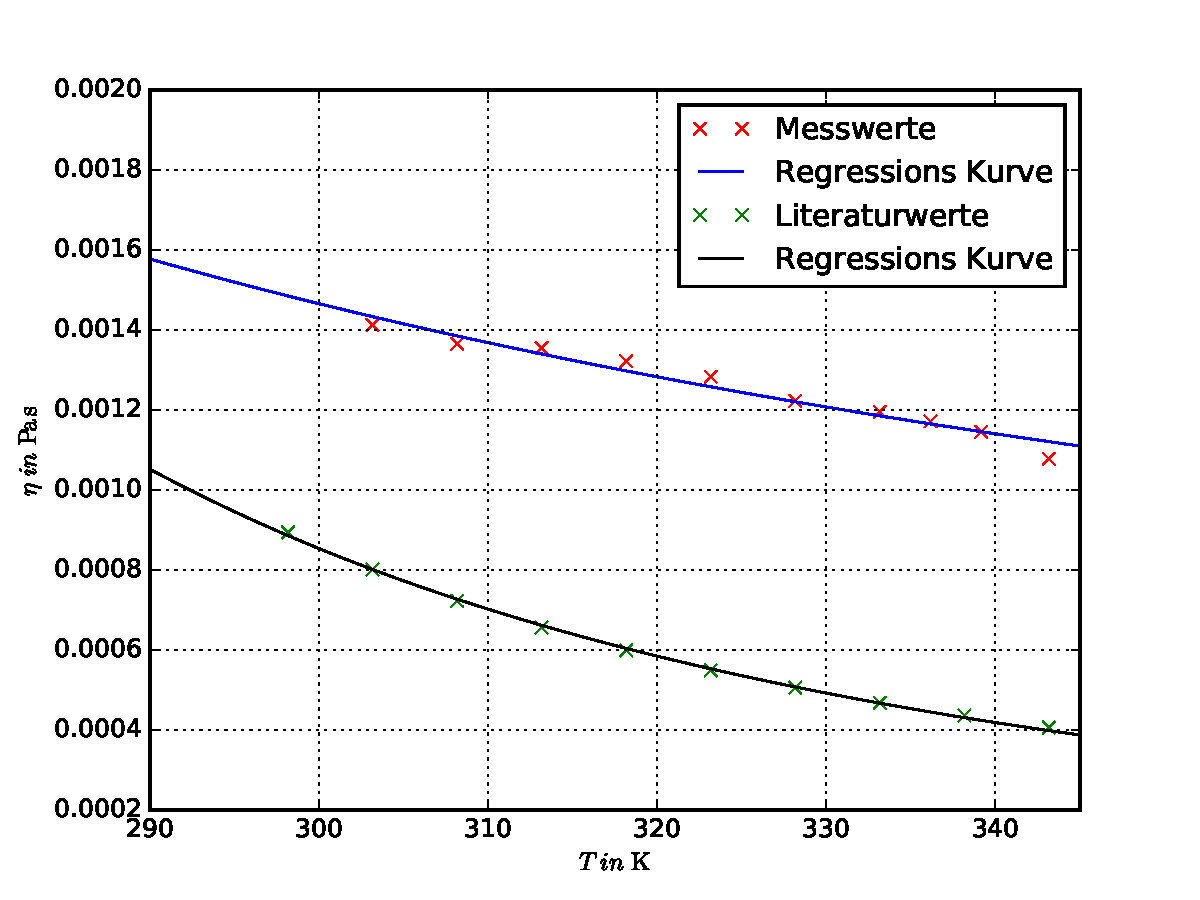
\includegraphics[width=0.75\textwidth]{pics/viskositaet_temp_mit_lit.pdf}
\caption{Temperatur gegen Viskosität}
\label{fig:t_v_v}
\end{figure}

\begin{figure}
\centering
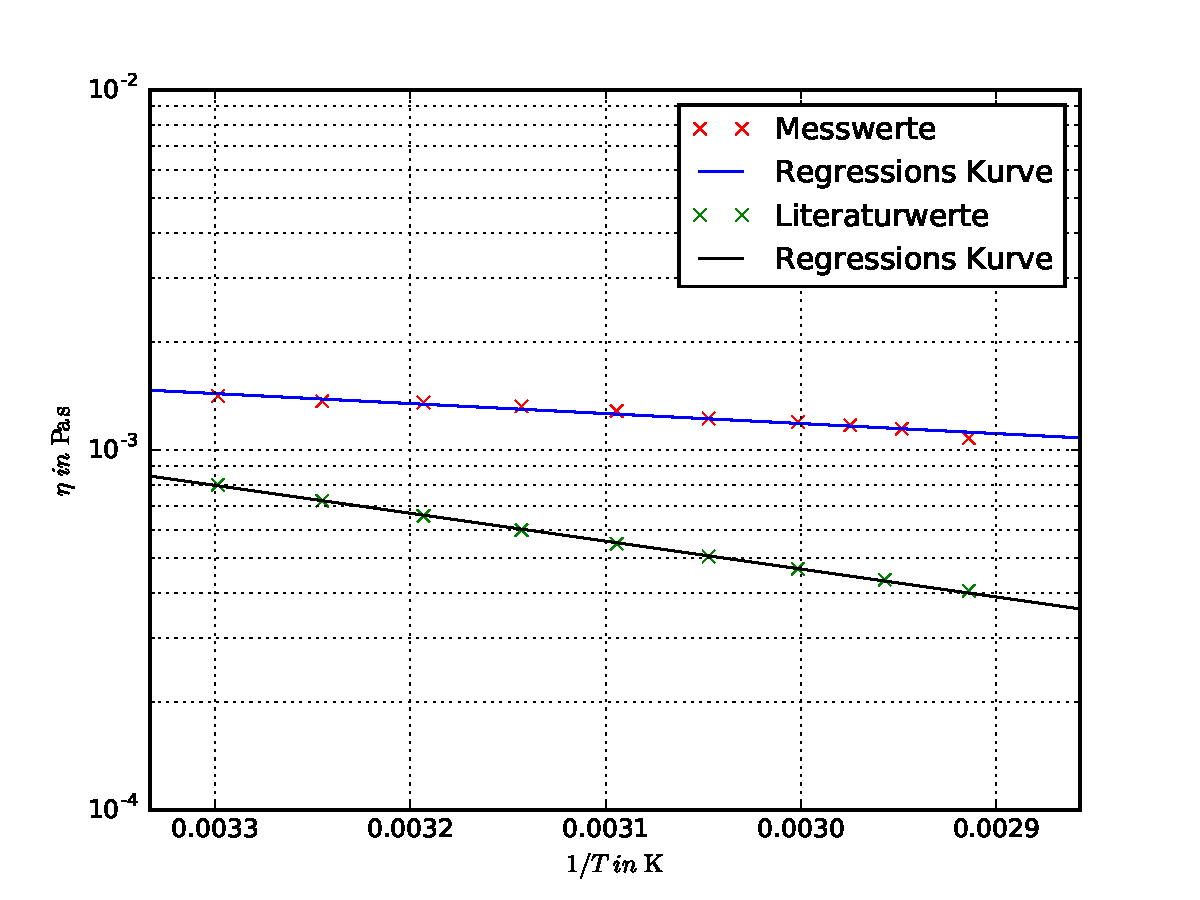
\includegraphics[width=0.75\textwidth]{pics/viskositaet_temp__log_mit_lit.pdf}
\caption{1/Temperatur gegen Viskosität (Halblogarithmische Skala)} %Überprüfen
\label{fig:t_v_l_v}
\end{figure}
\FloatBarrier

Hierbei wurde mittels der Python Bibliothek \emph{Scipy} eine %... ersetzen, scipy am besten mit \emph{} setzen
Regression an eine Funktion der Form $T_i = Ae^{\frac{B}{T}}$ bestimmt.
Als Parameter ergaben sich:
\begin{equation*}
A=\SI{1.74e-3}{\pascal\second}\quad B=\SI{6.4e2}{\kelvin} %Einheiten ?
\end{equation*}

\subsection{Bestimmung der Reynolds-Zahl}

Die \emph{Reynolds-Zahl} wird durch den Zusammenhang:

\begin{equation*}
\map{Re}=\frac{\rho v d}{\eta}
\end{equation*}
Dabei sei $d$ der Rohrdurchmesser und $v$ die Fallgeschindigkeit der Kugel.
Der Rohrdurchmesser wird durch den Durchmesser der großen Kugel angenährt.
Die Fallgeschwindigkeiten der Kugel bei den unterschiedlichen Temperaturen sind in Tabelle \ref{tab:fall_kugel} einzusehen.
Der Fehler der Geschwindigkeit ist in der Größenordnung $\num{e-6}$ und wird deshalb nicht mit aufgeslistet.

\begin{table}
\centering
\begin{tabular} {cc}
  \toprule
  Temperatur in $\si{\kelvin}$ & Fallgeschwindigkeit $v$ in $\si{\meter\per\second}$ \\
  \midrule 
  $\num{303.16}$ & $\num{0.00103}$ \\
  $\num{308.16}$ & $\num{0.00107}$ \\
  $\num{313.16}$ & $\num{0.00108}$ \\ 
  $\num{318.16}$ & $\num{0.00110}$ \\
  $\num{323.16}$ & $\num{0.00114}$ \\ 
  $\num{328.16}$ & $\num{0.0012}$ \\ 
  $\num{333.16}$ & $\num{0.00123}$ \\ 
  $\num{336.16}$ & $\num{0.001126}$ \\
  $\num{339.16}$ & $\num{0.00129}$ \\
  $\num{343.16}$ & $\num{0.00137}$ \\
\bottomrule
\end{tabular}
\caption{Fallgeschwindigkeit der großen Kugel bei unterschiedlichen Temperaturen}
\label{tab:fall_kugel}
\end{table}

Die sich damit ergebenen Werte für die \emph{Reynolds-Zahl} sind in Tabelle \ref{tab:rey_visko} 
zu finden.

\begin{table}
\centering
\begin{tabular} {cc}
  \toprule
  Temperatur in $\si{\kelvin}$ & \emph{Reynolds-Zahl} $\map{Re}$ \\
  \midrule 
  $\num{303.16}$ & $\num{11.1}\pm \num{0.03}$ \\
  $\num{308.16}$ & $\num{11.9}\pm \num{0.03}$ \\
  $\num{313.16}$ & $\num{12.1}\pm \num{0.04}$ \\ 
  $\num{318.16}$ & $\num{12.7}\pm \num{0.03}$ \\
  $\num{323.16}$ & $\num{13.4}\pm \num{0.03}$ \\ 
  $\num{328.16}$ & $\num{14.8}\pm \num{0.03}$ \\ 
  $\num{333.16}$ & $\num{15.5}\pm \num{0.03}$ \\ 
  $\num{336.16}$ & $\num{16.1}\pm \num{0.03}$ \\
  $\num{339.16}$ & $\num{16.8}\pm \num{0.07}$ \\
  $\num{343.16}$ & $\num{19}\pm \num{0.05}$ \\
\bottomrule
\end{tabular}
\caption{\emph{Reynolds-Zahl} des Viskosimeter bei unterschiedlichen Temperaturen}
\label{tab:rey_visko}
\end{table}